\documentclass[12pt]{article}
% Эта строка — комментарий, она не будет показана в выходном файле
\usepackage{ucs}
\usepackage[warn]{mathtext}
\usepackage[utf8x]{inputenc} % Включаем поддержку UTF8
\usepackage[russian]{babel}  % Включаем пакет для поддержки русского языка
\usepackage{amsmath}
\usepackage{mathtools}
\usepackage{amssymb}
% \usepackage[dvips]{graphicx}
% \graphicspath{{noiseimages/}}
\usepackage[pdftex]{graphicx}


% Параметры страницы: 1см от правого края и 2см от остальных.


\hoffset=0mm
\voffset=0mm
\textwidth=180mm        % ширина текста
\oddsidemargin=-6.5mm   % левое поле 25.4 - 5.4 = 20 мм
\textheight=240mm       % высота текста 297 (A4) - 40
\topmargin=-15.4mm      % верхнее поле (10мм)
\headheight=5mm      % место для колонтитула
\headsep=5mm          % отступ после колонтитула
\footskip=8mm         % отступ до нижнего колонтитула

\begin{document}
	\author {Жарков Андрей 495}
	\title {Лабораторная работа 5.2 \\  Интерференция света. Бипризма Френеля.}
    \maketitle{}
    
    \begin{center}
    	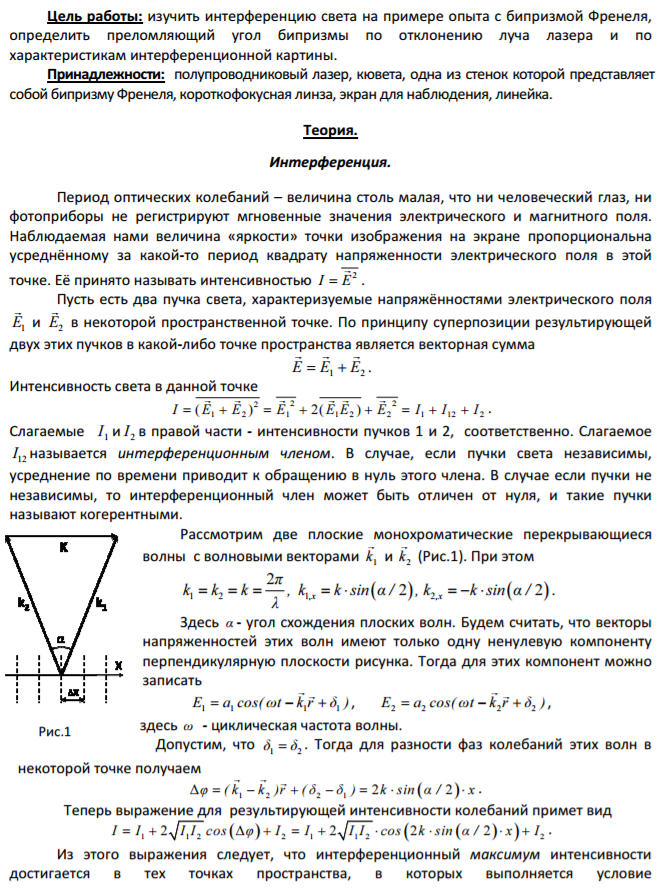
\includegraphics[width=13cm]{theory1.png}\\
    	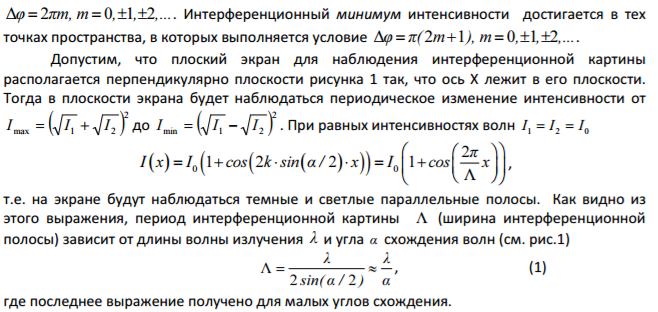
\includegraphics[width=15cm]{theory2.png}\\
    	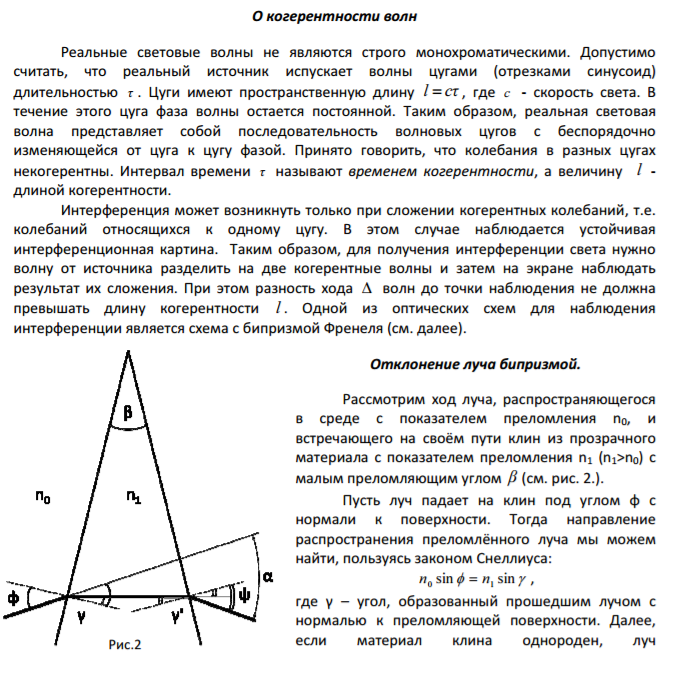
\includegraphics[width=15cm]{theory3.png}\\
    	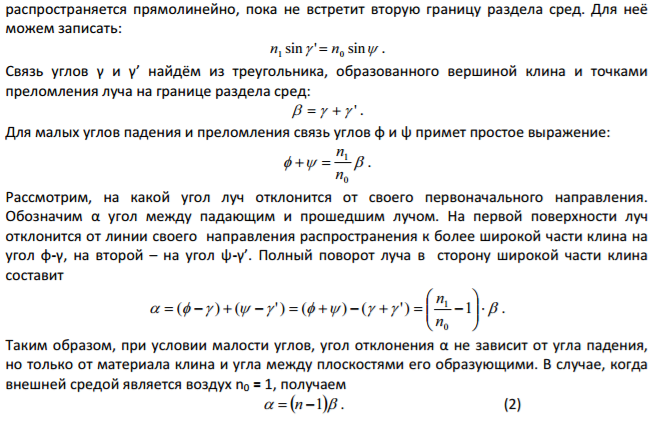
\includegraphics[width=16cm]{theory4.png}\\
    	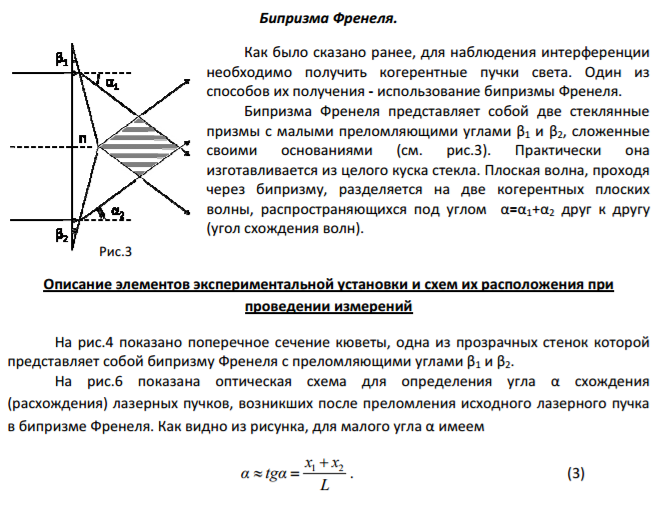
\includegraphics[width=16cm]{theory5.png}\\
    	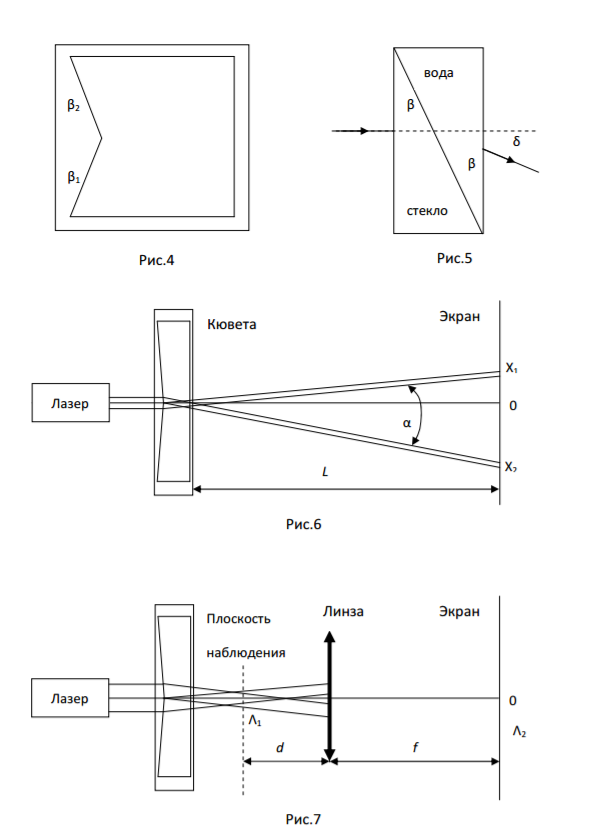
\includegraphics[width=13cm]{theory6.png}\\
    \end{center}
    
    \begin{center}
    	\textbf{\large Ход работы.}
    \end{center}
    
    1. Соберём схему, изображённую на рис. 6. Расстояние между лазером и кюветой порядка 5-10 см (меняется от опыта к опыту). Измеряя расстояние $x_1 + x_2$ и $L$, найдём угол $\alpha$ по формуле (3). Результаты измерений приведены в таблице:
    
    \begin{center}
    	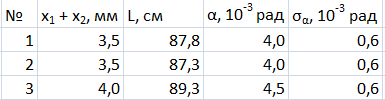
\includegraphics[width=8cm]{table1.png}
    \end{center}
    
    При измерениях $\sigma_{x_1 + x_2} = 0.5 мм$, что и вносит в результат наибольшую погрешность. Возьмём среднее значение угла $\alpha = (4,2 \pm 0,2) * 10^{-3}$ рад.\\
    
    2. Поставим линзу (F=36мм) между кюветой и экраном (см. рис. 7). При различном положении линзы измерим расстояние $f$ от линзы до экрана и период $\Lambda_2$ интерфереционной картины на экране. Пользуясь формулой тонкой линзы рассчитаем расстояние $d$ от линзы до плоскости наблюдения интерфереционной картины, а также увеличение $\Gamma$. Наконец, зная $\Gamma$ и $\Lambda_2$ найдём $\Lambda_1$ - период интерфереционной картины в плоскости наблюдения. По формуле (1), при $\lambda = 661 нм$, найдём угол $\alpha$. Результаты измерений и вычислений приведены в таблице:
    
    \begin{center}
    	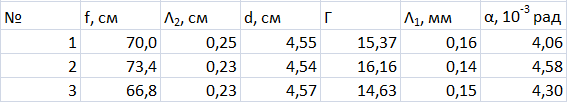
\includegraphics[width=12cm]{table2.png}
    \end{center}
    
    Относительная погрешность измерения $\varepsilon_{\Lambda_2} = 4\%$. Соответственно, такие же относительные погрешности у $\Lambda_1$ и угла $\alpha$. По формуле среднего арифметического найдём погрешность среднего значения $\alpha$. Итак: $$\alpha = (4,3 \pm 0,2) * 10^{-3} рад$$
    
    Вычислив разными способами угол $\alpha$ видим, что результаты в пределах погрешности совпадают.\\
    
    3. Нальём в кювету воды и повторим измерения. Получилось $f = 65,4см$, $\Lambda_2$ = 0,4см. Откуда $d=4,5см$, $\Gamma=14,3$, $\Lambda_1=0,28мм$, $\alpha=(2,4 \pm 0,1) * 10^{-3} рад$.
    
    Выражение для угла отклонения $\delta$ получить из закона преломления: $$n_{ст}sin\beta = n_в sin\gamma$$ $$n_в sin(\gamma - \beta) = sin\delta$$
    $$\delta = n_в \beta (\frac{n_{ст}}{n_в} - 1)$$
    
    Пользуясь этим найдём выражения для угла расхождения пучков с водой и без.
    $$\alpha_2 = \delta_1 + \delta_2 = (\beta_1 + \beta_2) (n_{ст} - n_в)$$
    $$\alpha_1 = (\beta_1 + \beta_2) (n_{ст} - 1)$$
    
    Откуда находим $n_{cт} = \frac{\alpha_2 / \alpha_1 - n_в}{\alpha_2 / \alpha_1 - 1} = 1,79 \pm 0,06$. Тяжёлый флинт?
    
    Среднее значение отклоняющего угла бипризмы $$\beta_{ср} = (\beta_1 + \beta_2) / 2 = \frac{\alpha_1}{n_{ст} - 1} = (5,3 \pm 0,2) * 10^{-3} рад$$
\end{document}